\section{Лекция 31.05.2018}

Аффинная система координат в $\RR^n$ определяется репЕром $(p, a_1, \dots, a_n)$, где $p \in \RR^n$ -- точка, $(e_1, \dots, e_n)$ -- базис $\RR^n$ (как векторного пространства).

\bigskip
Любая точка $x$ определяется однозначно своими координатами $(x_1, \dots, x_n)$ в этой аффинной системе координат (= в этом репере).

$x = p + x_1 e_1 + \dots + x_n e_n$

\bigskip
Пусть теперь $(p', e'_1, \dots, e'_n)$ -- другой репер

$(e'_1, \dots, e'_n) = (e_1, \dots, e_n) \cdot C, C \in M_n (\RR)$ -- матрицы перехода

$p' = p + \alpha_1 e_1 + \dots + \alpha_n e_n$

$x = p + x_1 e_1 + \dots + x_n e_n$

$x = p' + x'_1 e'_1 + \dots + x'_n e'_n$

\bigskip
\textbf{Предложение.} $\begin{pmatrix} x_1 \\ \vdots \\ x_n \end{pmatrix} = C \begin{pmatrix} x'_1 \\ \vdots \\ x'_n \end{pmatrix} + \begin{pmatrix} \alpha_1 \\ \vdots \\ \alpha_n \end{pmatrix}$

\bigskip
\textbf{\textit{Доказательство.}} $\rhd \ x = p + (e_1, \dots, e_n) \begin{pmatrix} x_1 \\ \vdots \\ x_n \end{pmatrix}$

$x = p' + (e'_1, \dots, e'_n) \begin{pmatrix} x'_1 \\ \vdots \\ x'_n \end{pmatrix} = p + (e_1, \dots, e_n) \begin{pmatrix} \alpha_1 \\ \vdots \\ \alpha_n \end{pmatrix} + (e_1, \dots, e_n) C \begin{pmatrix} x'_1 \\ \vdots \\ x'_n \end{pmatrix} \Leftrightarrow (e_1, \dots, e_n) \begin{pmatrix} x_1 \\ \vdots \\ x_n \end{pmatrix} = (e_1, \dots, e_n) \left(C \begin{pmatrix} x'_1 \\ \vdots \\ x'_n \end{pmatrix} + \begin{pmatrix} \alpha_1 \\ \vdots \\ \alpha_n \end{pmatrix}\right) \Rightarrow \begin{pmatrix} x_1 \\ \vdots \\ x_n \end{pmatrix} = C \begin{pmatrix} x'_1 \\ \vdots \\ x'_n \end{pmatrix} + \begin{pmatrix} \alpha_1 \\ \vdots \\ \alpha_n \end{pmatrix} \ \lhd$

\bigskip
\textbf{Определение.} Аффинная система координат называется \textit{прямоугольной декартовой системой координат (ПДСК)}, если в соответствующем репере базис $(e_1, \dots, e_n)$ является ортонормированным.

\bigskip
\textbf{Замечание.} Если есть ПДСК с репером $(p, e_1, \dots, e_n)$ и другая аффинная система координат с репером $(p', e'_1, \dots, e'_n)$, то вторая аффинная система координат будет ПДСК $\Leftrightarrow C$ ортогональная, где $(e'_1, \dots, e_n) = (e_1, \dots, e_n) C$

\subsection{Метрическая классификация гиперповерхностей второго порядка в $\RR^n$}

\textbf{Определение.} Множество $X \subseteq \RR^n$ называется \textit{квадрикой (или гиперповерхностью второго порядка)}, если в какой-либо аффинной системе координат она задается уравнением \begin{equation*}\overbrace{\sum\limits_{i=1}^n a_{ii} x_i^2 + \sum\limits_{1 \leqslant i < j \leqslant n} 2 a_{ij} x_i x_j}^{Q(x) \ квадратичная \ форма} + \overbrace{\sum\limits_{i=1} b_i x_i}^{l(x) \ линейная \ форма} + c = 0 (*)\end{equation*}

\bigskip
\textbf{Замечание.} $n = 2 \Rightarrow$ "коники" \ (от слова конус) или "кривые второго порядка"

$n = 3 \Rightarrow$ "поверхности второго порядка"

\bigskip
\textbf{Основная задача:} Найти новую ПДСК, в которой уравнение $(*)$ имеет простой вид.

\bigskip
\textbf{Теорема.} $\forall$ гиперповерхности второго порядка в $\RR^n \ \exists$ ПДСК, в которой уравнение $(*)$ имеет один из следующих видов:

\bigskip
\RomanNumeralCaps{1} (невырожденный случай)

$A_1 x_1^2 + \dots + A_n x_n^2 + c = 0, A_i = 0$

\bigskip
\RomanNumeralCaps{2} (вырожденный)

a) $A_1 x_1^2 + \dots + A_k x_k^2 + c = 0, k < n, A_i \neq 0$

б) $A_1 x_1^2 + \dots + A_k x_k^2 + B x_{k+1} = 0, k < n, A_i \neq 0, B \neq 0$

\bigskip
\textbf{\textit{Доказательство.}} $\rhd$ \underline{Шаг 1.} Переходя к новым координатам, приводим квадратичную форму $Q(x)$ к главным осям. В новых координатах уравнение $(*)$ будет иметь вид $A'_1 {x'_1}^2 + \dots + A'_n {x'_n}^2 + b'_1 x'_1 + \dots + b'_n x'_n + c' = 0$

\underline{Шаг 2.} Делаем замену: $x'_i = x''_i - \frac{b'_i}{2A'_i} \ \forall \ i$ с условием $A'_i \neq 0$, $x'_i = x''_i \ \forall \ i$ с условием $A'_i = 0$

В результате после перенумерации переменных получаем $A''_1 {x''_1}^2 + \dots + A''_k {x''_k}^2 + b''_{k+1} x''_{k+1} + \dots + b''_n x''_n + c'' = 0, k \leqslant n, A_i \neq 0$

Если $k = n$, то сразу получаем \RomanNumeralCaps{1}

Если $k < n$ и $b_i = 0$, то получаем \RomanNumeralCaps{2}а

Если $k < n$ и $\exists \ b''_i \neq 0$, то

\bigskip
\underline{Шаг 3.} Делаем замену

$\begin{cases} x''_i = x'_i \ при \ i \leqslant k \\ x''_{k+1} = \frac{1}{\sqrt[]{{b''_{k+1}}^2 + \dots + {b''_n}^2}}(b''_{k+1} x''_{k+1} + \dots + b''_n x''_n + c'') \\ 
x''_{k + 2} = \ \ \ любое \ дополнение \\ 
\vdots \ \ \ \ \ \ \ \  \ \ \ \ \ до \ ортоногонального \\
x''_n = \ \ \  \ \ \ \ \ \ \ базиса
\end{cases}$

В результате получаем \RomanNumeralCaps{2}б $\lhd$

\subsection{Канонические виды кривых второго порядка в $\RR^2$}

1) $\frac{x^2}{a^2} + \frac{y^2}{b^2} = 1, a\geqslant b > 0$ -- эллипс

\bigskip
2) $\frac{x^2}{a^2} + \frac{y^2}{b^2} = -1, a\geqslant b > 0$ -- мнимый эллипс

\bigskip
3) $\frac{x^2}{a^2} + \frac{y^2}{b^2} = 0, a\geqslant b > 0$ -- пара мнимых непересекающихся прямых

\bigskip
4) $\frac{x^2}{a^2} - \frac{y^2}{b^2} = 1$ -- гипербола

\bigskip
5) $\frac{x^2}{a^2} - \frac{y^2}{b^2} = 0, a, b > 0$ -- пара пересекающихся прямых

\bigskip
6) $y^2 = 2px, p > 0$ -- парабола

\bigskip
7) $x^2 = a^2, a > 0$ -- пара параллельных прямых

\bigskip
8) $x^2 = -a^2, a > 0$ -- пара мнимых параллельных прямых

\bigskip
9) $x^2 = 0$ -- пара совпадающих прямых

\bigskip
Картиночки:

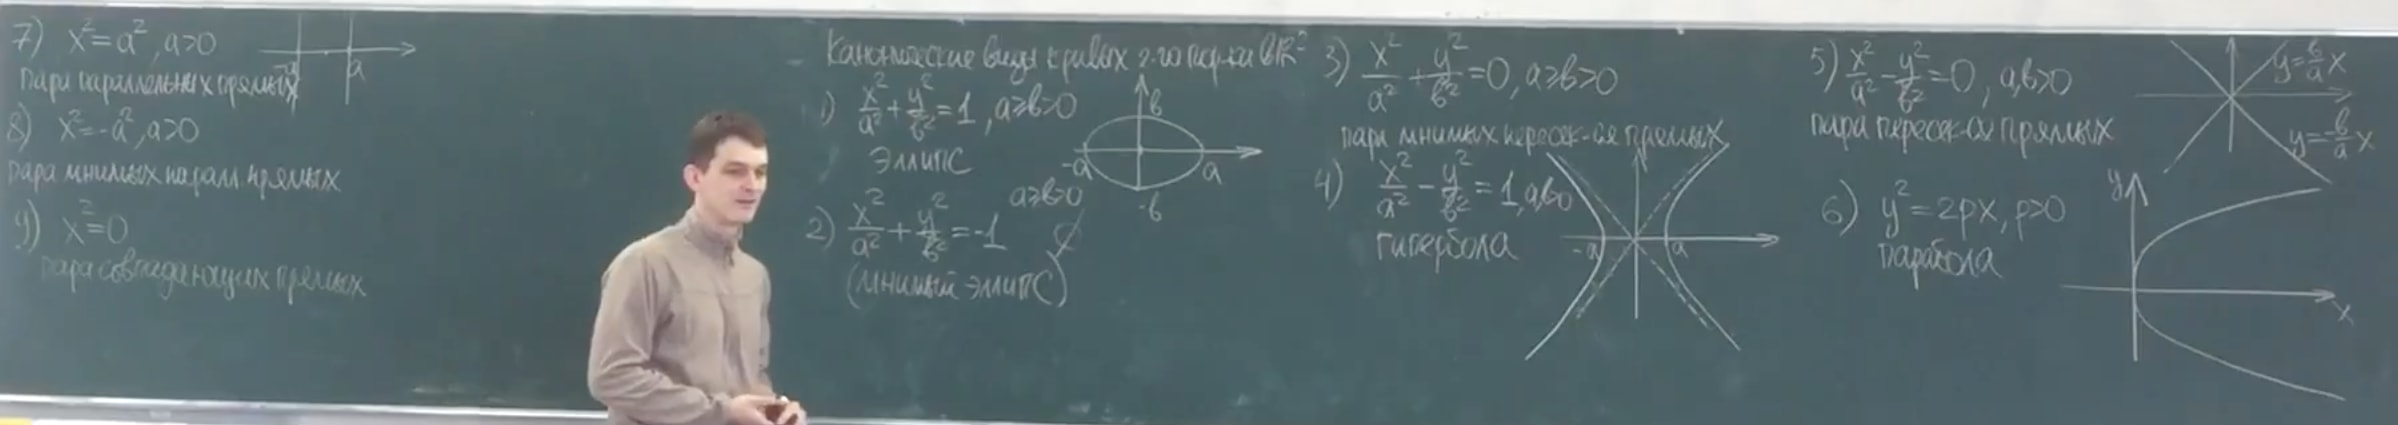
\includegraphics[width=19cm,height=15cm,keepaspectratio]{example2.jpg}

\subsection{Канонические виды поверхностей второго порядка в $\RR^3$}

1) $\frac{x^2}{a^2} + \frac{y^2}{b^2} + \frac{z^2}{c^2} = 1, a \geqslant b \geqslant c > 0$ -- эллипсоид

\bigskip
2) $\frac{x^2}{a^2} + \frac{y^2}{b^2} + \frac{z^2}{c^2} = -1$ -- мнимый эллипсоид

\bigskip
3) $\frac{x^2}{a^2} + \frac{y^2}{b^2} + \frac{z^2}{c^2} = 0$ -- вырожденный эллипсоид

\bigskip
4) $\frac{x^2}{a^2} + \frac{y^2}{b^2} - \frac{z^2}{c^2} = 1, a \geqslant b > 0, c > 0$ -- однополостный гиперболоид

\bigskip
5) $\frac{x^2}{a^2} + \frac{y^2}{b^2} - \frac{z^2}{c^2} = -1, a \geqslant b > 0, c > 0$ -- двуполостный гиперболоид

\bigskip
6) $\frac{x^2}{a^2} + \frac{y^2}{b^2} - \frac{z^2}{c^2} = 0, a \geqslant b > 0, c > 0$ -- эллиптический конус

\bigskip
7) $\frac{x^2}{a^2} + \frac{y^2}{b^2} = 2z$ -- эллиптический параболоид

\bigskip
8) $\frac{x^2}{a^2} - \frac{y^2}{b^2} = 2z$ -- гиперболический параболоид

\bigskip
9) $\frac{x^2}{a^2} + \frac{y^2}{b^2} = 1, a \geqslant b > 0$ -- эллиптический цилиндр

\bigskip
10) $\frac{x^2}{a^2} + \frac{y^2}{b^2} = -1$ -- мнимый эллиптический цилиндр

\bigskip
11) $\frac{x^2}{a^2} - \frac{y^2}{b^2} = 1$ -- гиперболический цилиндр

\bigskip
12) $y^2 = 2px, p > 0$ -- параболический цилиндр

\bigskip
13) $\frac{x^2}{a^2} - \frac{y^2}{b^2} = 0$ -- пара пересекающихся плоскостей

\bigskip
14) $\frac{x^2}{a^2} + \frac{y^2}{b^2} = 0$ -- пара мнимых пересекающихся плоскостей

\bigskip
15) $y^2 = a^2, a \neq 0$ -- пара параллельных плоскостей

\bigskip
16) $y^2 = -a^2, a \neq 0$ -- пара мнимых параллельных плоскостей

\bigskip
17) $y^2 = 0$ -- пара совпадающих плоскостей

